% ---------------------------------------------------------------
% TEMPLATE TCC1 - SENAC SANTO AMARO
% ---------------------------------------------------------------
% Trabalho de Conclusão de Curso 1
% Elaborado para apresentação da proposta inicial do TCC
% Estrutura: 4 capítulos (Introdução, Referencial Bibliográfico,
%            Desenvolvimento, Referências Bibliográficas)
% ---------------------------------------------------------------

\documentclass[
    12pt,                % tamanho da fonte
    openright,           % capítulos começam em página ímpar
    oneside,             % para impressão em apenas um lado do papel
    a4paper,             % tamanho do papel
    english,             % idioma adicional
    brazil               % idioma principal
]{abntex2}

% ---------------------------------------------------------------
% PACOTES
% ---------------------------------------------------------------
\usepackage{lmodern}                % Fonte Latin Modern
\usepackage[T1]{fontenc}            % Seleção de códigos de fonte
\usepackage[utf8]{inputenc}         % Codificação do documento
\usepackage{lastpage}               % Usado pela Ficha catalográfica
\usepackage{indentfirst}            % Indenta o primeiro parágrafo
\usepackage{color}                  % Controle de cores
\usepackage{graphicx}               % Inclusão de gráficos
\usepackage{microtype}              % Melhorias de justificação
\usepackage{float}                  % Para posicionamento de figuras
\usepackage{booktabs}               % Tabelas profissionais
\usepackage{multirow}               % Células mescladas em tabelas
\usepackage{longtable}              % Tabelas longas
\usepackage{amsmath,amssymb}        % Símbolos matemáticos
\usepackage{pgfgantt}               % Diagramas de Gantt
\usepackage[brazilian,hyperpageref]{backref}  % Páginas com citações
\usepackage[alf]{abntex2cite}       % Citações ABNT

% ---------------------------------------------------------------
% CONFIGURAÇÕES DO PDF
% ---------------------------------------------------------------
\makeatletter
\hypersetup{
    pdftitle={\@title},
    pdfauthor={\@author},
    pdfsubject={TCC1 - SENAC Santo Amaro},
    pdfcreator={LaTeX with abnTeX2},
    pdfkeywords={tcc}{senac}{santo amaro}{trabalho de conclusão},
    colorlinks=true,        % false: links em caixas; true: links coloridos
    linkcolor=blue,         % cor dos links internos
    citecolor=blue,         % cor dos links para bibliografia
    filecolor=magenta,      % cor dos links para arquivos
    urlcolor=blue,
    bookmarksdepth=4
}
\makeatother

% ---------------------------------------------------------------
% CONFIGURAÇÕES DE APARÊNCIA DO PDF FINAL
% ---------------------------------------------------------------
\definecolor{blue}{RGB}{41,5,195}

% ---------------------------------------------------------------
% TAMANHO DA FONTE DAS LEGENDAS (ABNT) -- 10 pt
% ---------------------------------------------------------------
% O título (\caption) e a linha de fonte (\legend) de figuras e
% tabelas devem ficar em 10 pt (o corpo do texto é 12 pt). Por
% padrão o memoir/abntex2 deixa essas legendas em 12 pt; os comandos
% abaixo reduzem o título e a fonte para 10 pt.
\renewcommand{\ABNTEXfontereduzida}{\fontsize{10}{12}\selectfont}
\captionnamefont{\ABNTEXfontereduzida}   % rótulo "Figura N"/"Tabela N"
\captiontitlefont{\ABNTEXfontereduzida}  % texto do título da legenda
\makeatletter
% Redefine \legend (usado em "Fonte: ...") para sair em 10 pt
% (a definição original do memoir fixa \normalsize = 12 pt).
\renewcommand{\legend}[1]{%
  \M@gettitle{#1}%
  \memlegendinfo{#1}%
  \par
  \begingroup
    \@parboxrestore
    \if@minipage
      \@setminipage
    \fi
    \ABNTEXfontereduzida
    \captiondelim{\mbox{}}%
    \@makecaption{}{\ignorespaces #1}\par
  \endgroup}
\makeatother

% ---------------------------------------------------------------
% INFORMAÇÕES DO DOCUMENTO
% ---------------------------------------------------------------
\titulo{Comparação entre CNN-BiLSTM e BiLSTM na classificação de fibrilação atrial em sinais de eletrocardiograma: análise do impacto da Cross-Entropy e da Focal Loss }
\author{Daniel de Araujo Carvalho \\ Eduardo Dias Santos}
\local{São Paulo}
\data{2026}
\orientador{Prof. Afonso Lelis}
% \coorientador{Prof. Nome do Coorientador} % Descomente se houver coorientador

\instituicao{%
  SENAC -- Serviço Nacional de Aprendizagem Comercial
  \par
  Unidade Santo Amaro
  \par
  Curso de Ciência da Computação
}

\tipotrabalho{Trabalho de Conclusão de Curso I}

\preambulo{Proposta de Trabalho de Conclusão de Curso apresentado ao SENAC Santo Amaro como requisito parcial para aprovação na disciplina de TCC1 do curso de Ciência da Computação.}

% ---------------------------------------------------------------
% COMPILA O ÍNDICE
% ---------------------------------------------------------------
\makeindex

% ---------------------------------------------------------------
% INÍCIO DO DOCUMENTO
% ---------------------------------------------------------------
\begin{document}

% Seleciona o idioma do documento
\selectlanguage{brazil}

% Retira espaço extra obsoleto entre as frases
\frenchspacing

% ---------------------------------------------------------------
% ELEMENTOS PRÉ-TEXTUAIS
% ---------------------------------------------------------------
\pretextual

% ---------------------------------------------------------------
% CAPA
% ---------------------------------------------------------------
\imprimircapa

% ---------------------------------------------------------------
% FOLHA DE ROSTO
% ---------------------------------------------------------------
\imprimirfolhaderosto

% ---------------------------------------------------------------
% RESUMO
% ---------------------------------------------------------------
\begin{resumo}
Este trabalho tem como objetivo analisar e comparar as arquiteturas de aprendizado profundo CNN-BiLSTM e BiLSTM na classificação de fibrilação atrial (FA) em sinais de eletrocardiograma (ECG), considerando o uso das funções de perda Cross-Entropy e Focal Loss. A justificativa para este estudo baseia-se na necessidade de investigar diferentes abordagens de aprendizado profundo para a classificação automática de sinais cardíacos, especialmente diante do desbalanceamento entre as classes presentes nos conjuntos de dados. O referencial bibliográfico abrange o processamento de sinais de ECG, a fibrilação atrial, redes neurais convolucionais, redes BiLSTM, funções de perda e métricas de avaliação de modelos de classificação. Como solução proposta, pretende-se desenvolver um estudo experimental utilizando o conjunto de dados PhysioNet/CinC Challenge 2017, comparando quatro configurações que combinam as duas arquiteturas com as duas funções de perda. A avaliação considerará métricas de desempenho da classificação e aspectos de custo computacional, como tempo de treinamento, tempo de inferência e quantidade de parâmetros. Este trabalho está organizado em capítulos que apresentam a introdução ao tema, o referencial bibliográfico que fundamenta a pesquisa, o desenvolvimento com a solução proposta e o cronograma de trabalho, seguidos das referências bibliográficas.

\vspace{\onelineskip}

\noindent
\textbf{Palavras-chave}: Eletrocardiograma. Fibrilação atrial. Aprendizado profundo. CNN-BiLSTM. BiLSTM.
\end{resumo}

% ---------------------------------------------------------------
% LISTA DE ILUSTRAÇÕES (FIGURAS)
% ---------------------------------------------------------------
% Gerada automaticamente a partir das \caption{} das figuras.
% Toda figura com legenda passa a constar nesta lista.
\pdfbookmark[0]{\listfigurename}{lof}
\listoffigures*
\cleardoublepage

% ---------------------------------------------------------------
% LISTA DE TABELAS
% ---------------------------------------------------------------
% Gerada automaticamente a partir das \caption{} das tabelas.
\pdfbookmark[0]{\listtablename}{lot}
\listoftables*
\cleardoublepage

% ---------------------------------------------------------------
% LISTA DE ABREVIATURAS E SIGLAS
% ---------------------------------------------------------------
% Esta lista deve vir antes do início do trabalho (elementos pré-textuais).
% Em ordem alfabética, relacione APENAS as abreviaturas e siglas que
% realmente aparecem no texto. Edite a tabela conforme o seu trabalho.
 


\pdfbookmark[0]{Lista de Abreviaturas e Siglas}{loas}
\chapter*{Lista de Abreviaturas e Siglas}

\noindent
A lista a seguir reúne as abreviaturas e siglas utilizadas neste trabalho, acompanhadas de seus respectivos significados.

\vspace{\onelineskip}

\begin{center}
\begin{tabular}{@{}p{3.2cm}p{0.6\textwidth}@{}}
\toprule
\textbf{Abreviatura/Sigla} & \textbf{Significado} \\
\midrule
AUC & \textit{Area Under the Curve} (Área sob a Curva) \\

CNN & \textit{Convolutional Neural Network} (Rede Neural Convolucional) \\

ECG & Eletrocardiograma \\

FA & Fibrilação Atrial \\

F1-score & Medida harmônica entre precisão e revocação \\

BiLSTM & \textit{Bidirectional Long Short-Term Memory} \\

LSTM & \textit{Long Short-Term Memory} \\

ROC & \textit{Receiver Operating Characteristic} \\


\bottomrule
\end{tabular}
\end{center}

\cleardoublepage

% ---------------------------------------------------------------
% SUMÁRIO
% ---------------------------------------------------------------
\pdfbookmark[0]{\contentsname}{toc}
\tableofcontents*
\cleardoublepage

% ---------------------------------------------------------------
% ELEMENTOS TEXTUAIS
% ---------------------------------------------------------------
\textual

% ===============================================================
% CAPÍTULO 1 - INTRODUÇÃO
% ===============================================================
\chapter{Introdução}
\label{cap:introducao}

O eletrocardiograma (ECG) é um exame utilizado para registrar a 
atividade elétrica do coração por meio de sensores posicionados 
sobre o corpo \cite{VanGelder2024}. A partir desse registro, 
é possível observar características relacionadas ao ritmo cardíaco 
e identificar possíveis alterações. Entre essas alterações está a 
fibrilação atrial (FA), uma arritmia caracterizada por atividade elétrica 
atrial desorganizada \cite{VanGelder2024}. Por esse motivo, a análise 
automatizada desses sinais tem sido estudada como uma aplicação de técnicas 
de aprendizado de máquina e aprendizado profundo \cite{Efe2024,AlMousa2023}.

Com o avanço do aprendizado profundo, diferentes arquiteturas de redes neurais 
passaram a ser utilizadas para analisar sinais de ECG. As Redes Neurais Convolucionais (CNN) 
podem identificar padrões locais presentes no sinal, enquanto as redes Long Short-Term Memory Bidirecionais (BiLSTM) 
são capazes de representar informações temporais considerando as duas direções da sequência. A combinação dessas abordagens, 
denominada CNN-BiLSTM, permite utilizar as camadas convolucionais para extrair características locais do sinal e as camadas 
BiLSTM para processar suas relações temporais.

Um dos desafios encontrados na classificação de ECG está relacionado ao desequilíbrio entre as classes. No conjunto de dados utilizado 
pelo PhysioNet/CinC Challenge 2017, por exemplo, existem 8.528 registros de ECG de uma derivação, sendo 5.154 classificados 
como ritmo normal e 771 como fibrilação atrial. Os registros possuem frequência de amostragem de 300 Hz e duração variável \cite{Clifford2017}.

Nesse cenário, além da escolha da arquitetura, a função utilizada durante o treinamento também pode influenciar o comportamento 
do modelo. A Cross-Entropy é uma função de perda amplamente utilizada em problemas de classificação, enquanto a Focal Loss 
foi proposta por Lin et al. (2017) para reduzir a contribuição dos exemplos mais fáceis durante o treinamento, direcionando 
maior atenção aos exemplos difíceis \cite{Lin2017}. Assim, a comparação entre essas funções pode ajudar a compreender 
seus efeitos em diferentes arquiteturas de classificação de ECG.

Dessa forma, este trabalho propõe uma comparação experimental entre as arquiteturas CNN-BiLSTM e BiLSTM, 
considerando as funções de perda Cross-Entropy e Focal Loss. O estudo será realizado sobre a classificação 
binária entre ritmo normal e fibrilação atrial, buscando analisar tanto o desempenho dos modelos quanto seu custo computacional.
%\vspace{0.3cm}
%\noindent\fbox{\parbox{\dimexpr\textwidth-2\fboxsep-2\fboxrule}{%
%\textbf{Orientação sobre a linguagem da introdução}

%\vspace{0.2cm}
%Escreva a \textbf{abertura} da introdução pensando em um \textbf{público amplo}, e não apenas na banca ou em especialistas. Um bom teste: alguém de outra área --- um colega de outro curso ou um familiar --- deveria entender, já nas primeiras linhas, qual é o assunto e por que ele importa.

%\vspace{0.2cm}
%\begin{itemize}
  %  \item \textbf{Do geral para o específico (técnica do ``funil'')}: parta do cenário cotidiano e vá afunilando, parágrafo a parágrafo, até o problema técnico que será investigado.
  %  \item \textbf{Evite jargão e siglas logo de início}; quando um termo técnico for inevitável, explique-o de forma simples na primeira vez em que aparecer.
 %   \item \textbf{Use exemplos concretos ou analogias} do dia a dia para tornar o tema palpável ao leitor leigo.
 %   \item \textbf{Reserve o aprofundamento técnico} para o Referencial Bibliográfico e o Desenvolvimento --- a introdução prepara o terreno, não esgota o assunto.
%\end{itemize}
%}}

% ---------------------------------------------------------------
\section{Contexto}
\label{sec:contexto}

A classificação automática de fibrilação atrial a partir de sinais de ECG apresenta 
um problema relevante para a área de Computação, pois envolve o processamento de séries 
temporais, a identificação de padrões e a classificação de dados. O próprio PhysioNet/CinC 
Challenge 2017 foi desenvolvido para estimular a criação de algoritmos capazes de classificar 
registros curtos de ECG em diferentes categorias, incluindo ritmo normal e fibrilação atrial \cite{Clifford2017}.

Além da variedade dos sinais, o desequilíbrio entre as classes pode dificultar o 
treinamento de modelos de aprendizado profundo. No conjunto de treinamento do desafio, 
a quantidade de registros de fibrilação atrial é consideravelmente menor que a quantidade 
de registros de ritmo normal \cite{Clifford2017}. Por esse motivo, torna-se importante 
avaliar o desempenho dos modelos por meio de diferentes métricas, e não apenas pela acurácia.

Nesse contexto, diferentes arquiteturas de aprendizado profundo podem apresentar comportamentos distintos ao 
lidar com as características dos sinais. A arquitetura BiLSTM permite processar informações temporais nas duas 
direções da sequência, enquanto a CNN-BiLSTM acrescenta uma etapa de extração de características locais antes desse 
processamento. Dessa forma, a comparação entre essas arquiteturas permite investigar se a inclusão de camadas convolucionais 
contribui para a classificação dos sinais de ECG. Da mesma forma, a função de perda utilizada no treinamento pode alterar a 
influência dos exemplos mais fáceis e difíceis sobre o aprendizado \cite{Lin2017}. Portanto, comparar arquiteturas e funções de 
perda sob condições experimentais controladas constitui uma forma de investigar quais fatores contribuem para o desempenho da classificação.

%\vspace{0.3cm}
%\noindent\fbox{\parbox{\dimexpr\textwidth-2\fboxsep-2\fboxrule}{%
%\textbf{Orientação sobre citações (ABNT NBR 10520:2023)}

%\vspace{0.2cm}
%O aluno deve \textbf{priorizar citações indiretas} (paráfrases), nas quais a ideia do autor é reescrita com as próprias palavras. Citações diretas (transcrições literais) \textbf{não são recomendadas}, exceto quando o texto original for insubstituível --- por exemplo, definições consagradas, leis, normas técnicas ou trechos cuja reformulação alteraria o sentido.

%\vspace{0.2cm}
%\textbf{Citação indireta} (recomendada) --- o autor interpreta e reescreve a ideia:

%\vspace{0.1cm}
%\textit{Exemplo 1 --- sistema autor-data entre parênteses:}\\
%A definição clara do problema é considerada um fator determinante para o sucesso de qualquer pesquisa na área de Computação \cite{Wazlawick2020}.

%\vspace{0.1cm}
%\textit{Exemplo 2 --- autor como parte do texto:}\\
%Para \citeonline{Pressman2016}, a escolha de uma metodologia adequada impacta diretamente na qualidade dos resultados obtidos em projetos de software.

%\vspace{0.2cm}
%\textbf{Citação direta curta} (até 3 linhas, apenas quando indispensável) --- entre aspas, com indicação de página:

%\vspace{0.1cm}
%Segundo \citeonline[p.~42]{Wazlawick2020}, ``a formulação do problema deve ser expressa de forma clara, objetiva e delimitada, evitando ambiguidades que possam comprometer o escopo da pesquisa''.

%\vspace{0.2cm}
%\textbf{Citação direta longa} (mais de 3 linhas, apenas quando indispensável) --- recuo de 4\,cm, fonte menor, sem aspas:

%\begin{citacao}
%A revisão bibliográfica não consiste em simplesmente listar os trabalhos encontrados, mas em analisá-los criticamente, identificando convergências, divergências e lacunas que justifiquem a realização de uma nova pesquisa \cite[p.~87]{Wazlawick2020}.
%\end{citacao}

%\textbf{Resumo}: use citações indiretas como regra. Reserve a citação direta para casos excepcionais em que a transcrição literal seja realmente necessária.
%}}

% ---------------------------------------------------------------
\section{Justificativa}
\label{sec:justificativa}
A justificativa acadêmica deste estudo está relacionada à comparação controlada de arquiteturas 
e funções de perda na identificação de fibrilação atrial (FA) em registros de ECG de derivação única. Estudos recentes investigaram o desbalanceamento entre classes de batimentos, 
a combinação de redes convolucionais e recorrentes e a Focal Loss
\cite{AlMousa2023,Efe2024,Albarrak2025}. Efe e Yavsan
compararam, inclusive, uma variante com entropia cruzada a outra com
Focal Loss em sua análise de componentes \cite{Efe2024}. Entretanto,
essas investigações classificam principalmente batimentos em bases
MIT-BIH e não respondem à comparação fatorial proposta para o ritmo de
registros curtos classificados como normais ou com FA no PhysioNet/CinC
2017. A classe FA e o problema de classificação por registro são
explicitamente descritos por Clifford et al. \cite{Clifford2017}.
Assim, o diferencial deste trabalho é estimar, na mesma base e sob o mesmo
protocolo, como a presença da etapa CNN e a escolha da função de perda
afetam o F1 da classe FA e o custo computacional, sem tomar os resultados
por batimento dos estudos citados como referência numérica direta.

Nesse contexto, a escolha das arquiteturas CNN-BiLSTM e BiLSTM busca investigar a contribuição da extração de 
características locais realizada pelas camadas convolucionais. Enquanto a BiLSTM processa informações temporais 
considerando as duas direções da sequência, a CNN-BiLSTM incorpora uma etapa convolucional antes desse processamento. 
Como ambas utilizam uma estrutura recorrente bidirecional, sua comparação permite analisar a possível contribuição 
dessa etapa adicional para a identificação de fibrilação atrial.

Outra questão relevante está relacionada ao desbalanceamento entre as classes de ritmo normal e fibrilação atrial. 
A menor quantidade de registros de fibrilação atrial pode dificultar a identificação dessa classe pelos modelos. 
Nesse cenário, investigar a influência das funções de perda Cross-Entropy e Focal Loss é importante para compreender 
se diferentes estratégias de aprendizado contribuem para melhorar a classificação da classe minoritária.

Do ponto de vista prático, a pesquisa também se justifica pela necessidade de considerar os recursos computacionais 
exigidos pelas arquiteturas. Modelos mais complexos podem apresentar custos adicionais de treinamento e inferência, 
tornando relevante investigar se possíveis melhorias no desempenho são acompanhadas de maior demanda computacional. 
Assim, a contribuição pretendida deste trabalho consiste em oferecer uma comparação experimental controlada entre 
CNN-BiLSTM e BiLSTM, considerando diferentes funções de perda, a identificação de fibrilação atrial e o equilíbrio 
entre desempenho e custo computacional.
% ---------------------------------------------------------------
\section{Objetivo}
\label{sec:objetivo}

Os objetivos a seguir delimitam o escopo prático e analítico do estudo, orientando a condução dos experimentos e a interpretação dos resultados obtidos.

\subsection{Objetivo principal}

Analisar experimentalmente e comparar as arquiteturas de aprendizado profundo CNN-BiLSTM e BiLSTM para a 
classificação de fibrilação atrial em sinais de eletrocardiograma, avaliando o impacto das funções de perda 
Cross-Entropy e Focal Loss por meio de métricas de desempenho e custo computacional.


\subsection{Objetivos secundários}

\begin{enumerate}
    \item Realizar o pré-processamento dos sinais de ECG do conjunto PhysioNet/CinC 2017, considerando as classes Normal e Fibrilação Atrial;
    \item Implementar e treinar as duas arquiteturas propostas, CNN-BiLSTM e BiLSTM, utilizando as funções de perda Cross-Entropy e Focal Loss;
    \item Avaliar e comparar o desempenho das quatro configurações experimentais por meio de Accuracy, Precision, Recall, Specificity, F1-score e matriz de confusão;
    \item Analisar o impacto das funções de perda Cross-Entropy e Focal Loss, especialmente sobre a classificação da classe minoritária de Fibrilação Atrial;
    \item Comparar o custo computacional das abordagens, considerando tempo de treinamento, tempo de inferência e quantidade de parâmetros, identificando a configuração com melhor relação entre desempenho e custo computacional.
\end{enumerate}


% ===============================================================
% CAPÍTULO 2 - REFERENCIAL BIBLIOGRÁFICO
% ===============================================================
\chapter{Referencial Bibliográfico}
\label{cap:referencial}

Este capítulo reúne os fundamentos clínicos e computacionais necessários à comparação entre as arquiteturas CNN-BiLSTM e BiLSTM na classificação de registros de eletrocardiograma (ECG). A Seção~\ref{sec:metodologia_bibliografica} descreve o levantamento das fontes; a Seção~\ref{sec:referencial} apresenta os conceitos utilizados no estudo; e a Seção~\ref{sec:trabalhos_relacionados} examina pesquisas recentes pertinentes às escolhas metodológicas deste trabalho.

\section{Metodologia da pesquisa bibliográfica}
\label{sec:metodologia_bibliografica}

Foi realizado um levantamento bibliográfico exploratório de publicações sobre classificação de sinais de ECG, fibrilação atrial (FA), arquiteturas recorrentes e convolucionais, funções de perda e avaliação em dados desbalanceados. Foram consultados registros do PubMed, a documentação e o artigo do desafio PhysioNet/Computing in Cardiology 2017 e artigos publicados nos periódicos \textit{Digital Health}, \textit{Mathematical Biosciences and Engineering} e \textit{Sensors}. As buscas exploratórias utilizaram, entre outras, as seguintes combinações de termos em inglês:
\begin{itemize}
    \item \textit{``atrial fibrillation'' AND ``single-lead ECG'' AND ``deep learning''};
    \item \textit{``focal loss'' AND ``ECG'' AND ``class imbalance''};
    \item \textit{``ECG'' AND ``CNN'' AND ``BiLSTM'' AND ``focal loss''};
    \item \textit{``heartbeat classification'' AND ``class imbalance'' AND ``ECG''}.
\end{itemize}

Para a seção de trabalhos relacionados, foram escolhidos três artigos originais em inglês publicados entre 2023 e 2025, relevantes para pelo menos um dos eixos desta pesquisa: desbalanceamento de classes, combinação de redes convolucionais e recorrentes ou comparação de funções de perda. A seleção considerou títulos, resumos, métodos, bases e classes avaliadas. Os três estudos tratam principalmente de classificação de batimentos, não da classificação binária de FA por registro proposta neste TCC. O artigo de Clifford et al. (2017) foi mantido como fonte específica da tarefa e da base PhysioNet/CinC 2017 \cite{Clifford2017}. Para fundamentar conceitos e escolhas de projeto, foram incluídas também publicações anteriores, inclusive estudos sobre CNN, LSTM e validação de classificadores.

Este levantamento tem caráter exploratório: a seleção dos três trabalhos permite contextualizar partes do problema, mas não constitui uma revisão sistemática nem pretende enumerar todos os estudos existentes. Como esses artigos classificam batimentos em outras bases, seus números não constituem resultados de referência para o F1 da classe FA no recorte binário deste trabalho.

\section{Referencial}
\label{sec:referencial}

\subsection{Eletrocardiograma e fibrilação atrial}
\label{subsec:ecg_fa}

O ECG registra a atividade elétrica cardíaca ao longo do tempo. Na avaliação do ritmo, a fibrilação atrial está associada à ausência de ondas P discerníveis e repetitivas e à irregularidade da ativação ventricular, observável na variação dos intervalos RR entre batimentos. Esses indícios precisam ser interpretados no contexto do traçado, pois irregularidades também podem ocorrer em outros ritmos e o ruído pode prejudicar a análise \cite{VanGelder2024,Clifford2017}.

O PhysioNet/Computing in Cardiology Challenge 2017 disponibilizou registros curtos de ECG de uma derivação, classificados como ritmo normal, fibrilação atrial, outro ritmo ou ruidoso. Na versão inicial dos rótulos descrita por \citeonline{Clifford2017}, o conjunto público de treinamento possui 8.528 registros: 5.154 normais, 771 com FA, 2.557 de outros ritmos e 46 ruidosos. O recorte deste TCC considera apenas normal e FA dessa versão, totalizando 5.925 registros antes da divisão em treino, validação e teste. A razão entre as duas classes nesse recorte é aproximadamente 6,7 para 1, o que caracteriza o desbalanceamento a ser investigado. Os resultados obtidos nesse problema binário não podem ser tratados como pontuação oficial do desafio, que considera outras categorias.

\subsection{Aprendizado profundo e redes convolucionais para ECG}
\label{subsec:cnn_ecg}

Uma série temporal contém observações ordenadas; no ECG, a posição e a evolução dos padrões ao longo do registro são relevantes para a classificação do ritmo. No aprendizado profundo, as características úteis à tarefa podem ser aprendidas a partir dos dados. Redes convolucionais unidimensionais (CNN 1D) aplicam filtros ao longo do sinal para aprender características locais. Essa abordagem foi utilizada tanto isoladamente quanto em combinação com camadas recorrentes na classificação de ECG \cite{Goodfellow2016,Zihlmann2017,Xiong2018}.

\subsection{Redes recorrentes, LSTM e BiLSTM}
\label{subsec:rnn_bilstm}

Redes neurais recorrentes (RNN) processam uma sequência mantendo uma representação que depende das posições já percorridas. Essa estrutura permite modelar relações temporais entre as características extraídas do ECG \cite{Goodfellow2016,Xiong2018}.

As redes \textit{Long Short-Term Memory} (LSTM) foram propostas para lidar com dificuldades de aprendizagem de relações distantes em sequências por meio de mecanismos de memória controlados por portas \cite{Hochreiter1997}. Em uma estrutura bidirecional, a sequência é processada em ambos os sentidos, de modo que a representação de uma posição pode incorporar informações anteriores e posteriores \cite{Schuster1997}. A BiLSTM emprega células LSTM nessas duas direções; como este estudo classifica registros completos, os dois sentidos do sinal estão disponíveis no momento da predição \cite{Cheng2021}.

Neste trabalho, a BiLSTM processará diretamente a sequência de entrada, enquanto a CNN-BiLSTM terá uma etapa convolucional antes do bloco recorrente bidirecional. As duas propostas compartilham o tipo de componente temporal, permitindo investigar a contribuição da extração convolucional para a tarefa definida. Para interpretar essa comparação, o protocolo experimental deverá explicitar a forma de entrada, as dimensões das camadas e o número de parâmetros de cada rede.

\subsection{Desbalanceamento de classes e funções de perda}
\label{subsec:funcoes_perda}

Em uma tarefa binária, o modelo atribui a cada registro uma probabilidade de pertencer à classe positiva, aqui definida como FA. Seja $y\in\{0,1\}$ o rótulo verdadeiro e $p\in(0,1)$ a probabilidade prevista para FA. A probabilidade atribuída à classe verdadeira é $p_t=p$ quando $y=1$ e $p_t=1-p$ quando $y=0$. A entropia cruzada binária para um exemplo pode então ser escrita como \cite{Goodfellow2016,Lin2017}
\begin{equation}
    \mathcal{L}_{\mathrm{CE}}(p_t)=-\log(p_t).
    \label{eq:ce_binaria}
\end{equation}

Na entropia cruzada não ponderada, cada exemplo contribui segundo a probabilidade atribuída ao seu rótulo. Como a base contém mais registros normais que registros com FA, é necessário verificar empiricamente se o treinamento resultante reconhece adequadamente a classe menos frequente. A \textit{Focal Loss}, proposta inicialmente para enfrentar o predomínio de exemplos fáceis em detecção de objetos, acrescenta um fator que reduz a contribuição relativa dos exemplos bem classificados \cite{Lin2017}:
\begin{equation}
    \mathcal{L}_{\mathrm{FL}}(p_t)=-\alpha_t(1-p_t)^{\gamma}\log(p_t),
    \label{eq:focal_binaria}
\end{equation}
em que $\gamma\geq0$ controla a ênfase nos exemplos difíceis. Na variante com ponderação de classes, $\alpha_t=\alpha$ quando $y=1$ (FA) e $\alpha_t=1-\alpha$ quando $y=0$ (normal), para $\alpha\in[0,1]$ \cite{Lin2017}. Sem ponderação, pode-se definir $\alpha_t=1$ para ambas as classes: nesse caso, $\gamma=0$ faz a Equação~\ref{eq:focal_binaria} coincidir com a entropia cruzada não ponderada da Equação~\ref{eq:ce_binaria}. Com pesos de classe, $\gamma=0$ produz a entropia cruzada ponderada. A Focal Loss não garante, por si só, melhor identificação de FA; essa hipótese será examinada nas quatro combinações entre arquitetura e função de perda.

\subsection{Métricas para classificação desbalanceada}
\label{subsec:metricas}

Para avaliar as previsões, FA será considerada a classe positiva. Na matriz de confusão, verdadeiros positivos (VP) são registros com FA corretamente identificados, falsos negativos (FN) são registros com FA classificados como normais, falsos positivos (FP) são registros normais classificados como FA e verdadeiros negativos (VN) são registros normais corretamente classificados. A partir dessas quantidades, serão utilizadas as métricas
\begin{align}
    \text{Precisão} &= \frac{VP}{VP+FP}, \nonumber\\
    \text{Revocação} &= \frac{VP}{VP+FN}, \nonumber\\
    \text{Especificidade} &= \frac{VN}{VN+FP}, \nonumber\\
    \text{Acurácia} &= \frac{VP+VN}{VP+VN+FP+FN}, \nonumber\\
    F_1 &= \frac{2\,\text{Precisão}\,\text{Revocação}}{\text{Precisão}+\text{Revocação}}. \label{eq:metricas}
\end{align}

A revocação, também chamada sensibilidade, indica a fração dos registros com FA recuperada pelo modelo; a precisão informa a fração de previsões de FA que está correta. O $F_1$ sintetiza precisão e revocação, enquanto a especificidade descreve o acerto entre os registros normais. Como a acurácia pode ser elevada mesmo diante de dificuldades com a classe menos frequente, as métricas serão apresentadas em conjunto \cite{Saito2015}.

Também serão consideradas a área sob a curva ROC (AUC-ROC) e a área sob a curva precisão--revocação (AUC-PR), obtidas a partir de diferentes limiares de decisão. A curva precisão--revocação merece atenção particular na presença de desbalanceamento, pois torna visível a relação entre falsos positivos e a recuperação da classe FA \cite{Saito2015}. Sua interpretação deverá levar em conta a proporção de FA no conjunto de teste.

\section{Trabalhos relacionados}
\label{sec:trabalhos_relacionados}

Foram escolhidos três estudos recentes que tratam de classificação de batimentos em ECG e abordam aspectos metodológicos pertinentes ao presente trabalho: desbalanceamento de classes, arquitetura híbrida e função de perda. Eles não classificam registros do PhysioNet/CinC 2017 na tarefa binária normal versus FA. A tarefa de distinguir FA de outros ritmos em registros curtos de uma derivação é descrita por \citeonline{Clifford2017}; neste TCC, será adotado um recorte binário dessa base. Assim, a aproximação entre os três estudos a seguir e a proposta é metodológica, não uma equivalência entre classes, unidades de análise ou resultados numéricos.

\subsection{Al-Mousa et al. (2023)}
\label{subsec:trab_almousa}

\cite{AlMousa2023} investigaram a classificação de cinco categorias de batimentos (N, SVEB, VEB, F e Q) com ênfase nas classes raras F e Q. A base principal foi a \textit{MIT-BIH Supraventricular Arrhythmia Database}; foram comparados cinco classificadores tradicionais, incluindo regressão logística e \textit{Random Forest}, com técnicas de balanceamento por SMOTE e incorporação de exemplos de outras bases. Os autores relataram acurácia de 97\% para o melhor classificador e revocação de apenas 30\% para a classe Q nesse resultado. Isso ilustra por que uma acurácia global elevada não dispensa a análise da classe minoritária. O estudo não empregou CNN-BiLSTM nem definiu FA como classe positiva de um registro inteiro. Neste TCC, a importância das classes minoritárias será examinada pelo F1 e pela revocação da classe FA em registros do CinC 2017, sem importar os resultados por batimento como parâmetro de desempenho.

\subsection{Efe e Yavsan (2024)}
\label{subsec:trab_efe}

\cite{Efe2024} propuseram a arquitetura \textit{AttBiLFNet}, que combina CNN, BiLSTM, mecanismo de atenção e \textit{Focal Loss} na classificação de cinco classes de batimentos da \textit{MIT-BIH Arrhythmia Database}: normal (N), bloqueio de ramo esquerdo (LBBB), bloqueio de ramo direito (RBBB), contração ventricular prematura (PVC) e batimento atrial prematuro (APB). Os autores avaliaram configurações alternativas, incluindo a substituição da \textit{Focal Loss} por entropia cruzada categórica, e empregaram validação cruzada em dez partes. Portanto, a comparação entre essas duas perdas já foi explorada para batimentos de ECG. Entretanto, APB não equivale à fibrilação atrial, e o artigo não examina o desenho fatorial CNN-BiLSTM versus BiLSTM, cruzado com as duas perdas, para a classificação binária de FA por registro. Seus resultados não serão comparados numericamente ao F1 de FA deste TCC.

\subsection{Albarrak, Alharbi e Ibrahim (2025)}
\label{subsec:trab_albarrak}

\cite{Albarrak2025} compararam modelos de aprendizado de máquina e redes neurais para classificar cinco classes de batimentos da base MIT-BIH. A proposta combina CNN 1D e LSTM, com otimização de hiperparâmetros por \textit{Grey Wolf Optimizer}, e alcançou acurácia global de 97\% no protocolo relatado. Os autores destacam a ausência de validação cruzada e testes estatísticos como limitação. O artigo motiva a análise conjunta de desempenho e custo de modelos híbridos, mas utiliza LSTM, não BiLSTM, e não classifica FA em registros curtos do CinC 2017. Sua acurácia não será usada como meta numérica para a presente tarefa.

A Tabela~\ref{tab:trabalhos_relacionados} resume os recortes metodológicos. A lacuna examinada neste TCC não é a ausência de estudos com CNN, BiLSTM ou \textit{Focal Loss} em ECG: Efe e Yavsan já combinaram esses componentes e compararam perdas em uma análise de batimentos. O diferencial proposto é investigar, em um protocolo comum, como a presença da etapa CNN e a escolha da perda afetam o F1 da classe FA quando a unidade de avaliação é um registro de ECG de derivação única do CinC 2017. Também será medido o custo computacional das quatro configurações. Essas comparações internas não permitem concluir que os modelos superam os resultados publicados nas outras bases.

\begin{table}[htbp]
    \centering
    \caption{Comparação entre trabalhos relacionados e a proposta deste TCC}
    \label{tab:trabalhos_relacionados}
    \ABNTEXfontereduzida
    \begin{tabular}{@{}p{2.6cm}p{4.3cm}p{5.9cm}@{}}
        \toprule
        \textbf{Estudo} & \textbf{Base e unidade} & \textbf{Método e relação com este TCC} \\
        \midrule
        Al-Mousa et al. (2023) & MIT-BIH supraventricular; cinco classes de batimentos & Métodos tradicionais, SMOTE e combinação de bases; evidencia dificuldade nas classes raras, sem classificar FA por registro \\
        \addlinespace
        Efe e Yavsan (2024) & MIT-BIH Arrhythmia; cinco classes de batimentos & CNN--BiLSTM com atenção e \textit{Focal Loss}; analisa entropia cruzada como alternativa, sem avaliar FA por registro \\
        \addlinespace
        Albarrak et al. (2025) & MIT-BIH; cinco classes de batimentos & CNN--LSTM com otimização GWO; relata custo e reconhece falta de validação estatística \\
        \addlinespace
        Este TCC & CinC 2017; registro normal ou FA & BiLSTM vs. CNN--BiLSTM cruzadas com entropia cruzada vs. \textit{Focal Loss}; F1 de FA e custo \\
        \bottomrule
    \end{tabular}
    \legend{Fonte: Elaborado pelos autores (2026), com base em \cite{AlMousa2023}, \cite{Efe2024} e \cite{Albarrak2025}.}
\end{table}

% ===============================================================
% CAPÍTULO 3 - DESENVOLVIMENTO
% ===============================================================
\chapter{Desenvolvimento}
\label{cap:desenvolvimento}

% Neste capítulo, apresenta-se a solução proposta para o problema identificado, bem como o cronograma de trabalho previsto para o desenvolvimento completo do projeto no TCC2.

% ---------------------------------------------------------------
\section{Solução proposta}
\label{sec:solucao}


\subsection{Visão geral da solução}

O desenvolvimento da solução será organizado em etapas, iniciando pela aquisição e preparação dos sinais de ECG, seguida pela implementação das arquiteturas de redes neurais, 
treinamento, validação e avaliação dos resultados.

Inicialmente, serão selecionados os registros correspondentes às classes Normal e Fibrilação Atrial da base PhysioNet/CinC Challenge 
2017. Em seguida, os sinais passarão por procedimentos de pré-processamento, necessários para adequar os registros às entradas das redes neurais.

Após a preparação dos dados, serão implementadas as arquiteturas CNN-BiLSTM e BiLSTM. Cada arquitetura será treinada utilizando as duas 
funções de perda selecionadas, resultando em quatro configurações experimentais.

Por fim, os resultados serão comparados considerando métricas de desempenho, análise estatística e custo computacional. Essa abordagem 
permitirá investigar os efeitos individuais das arquiteturas e das funções de perda, bem como a interação entre esses dois fatores.


\subsection{Arquitetura da solução}

A arquitetura da solução será organizada em um fluxo de processamento composto por aquisição dos dados, seleção das classes, pré-processamento, 
divisão dos conjuntos de dados, treinamento dos modelos e avaliação dos resultados.

A Figura~\ref{fig:arquitetura} apresenta uma representação geral do fluxo proposto para o desenvolvimento do experimento.

\begin{figure}[htb]
    \centering
    \caption{Arquitetura proposta para o sistema de classificação de sinais ECG.}
    \label{fig:arquitetura}
    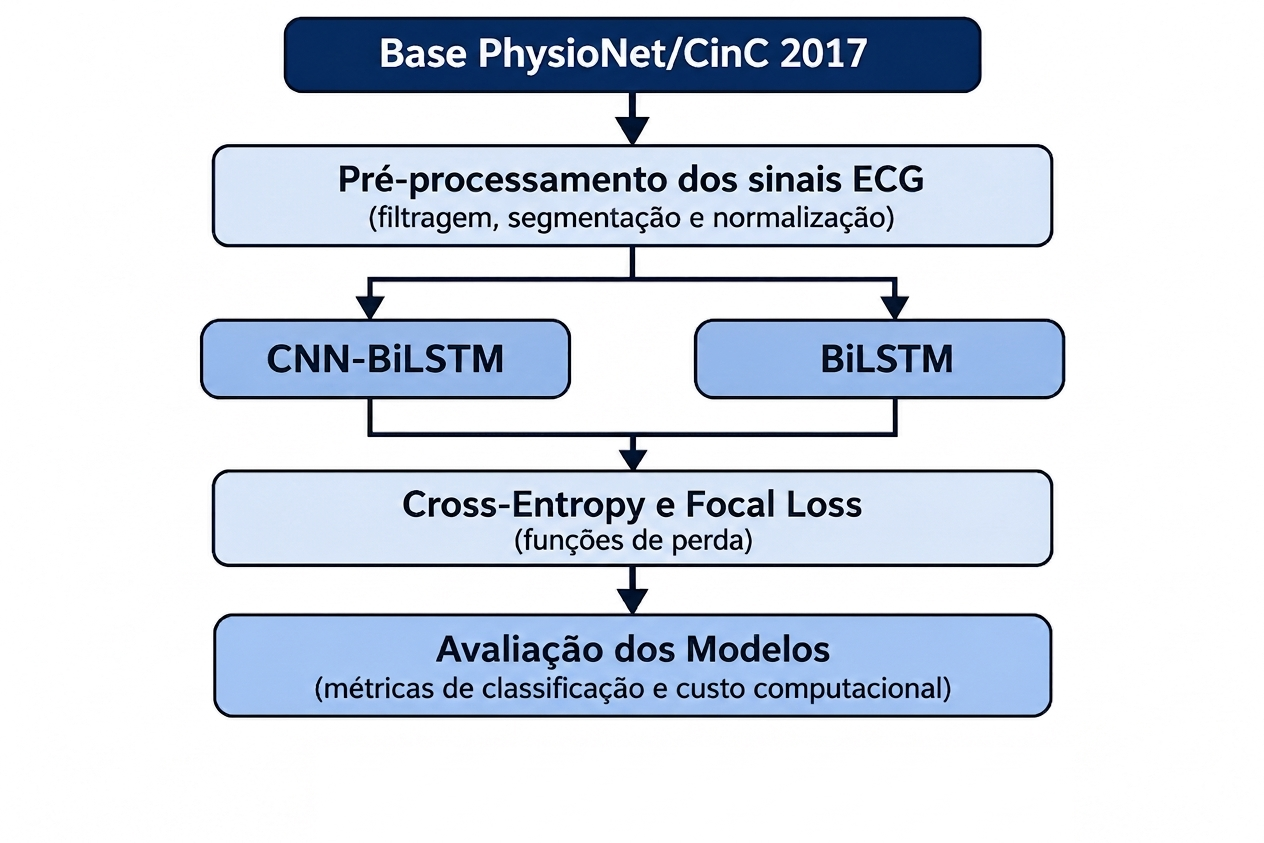
\includegraphics[width=0.75\textwidth]{assets/fluxograma_tcc.jpg}
    \legend{Fonte: Elaborado pelos autores (2026)}
\end{figure}

Conforme apresentado na Figura~\ref{fig:arquitetura}, inicialmente serão obtidos os registros de ECG da base PhysioNet/CinC Challenge 2017. 
Na sequência, serão selecionados os registros pertencentes às classes Normal e Fibrilação Atrial, excluindo-se as categorias Outro Ritmo e Ruidoso.

Após essa seleção, os sinais serão submetidos ao pré-processamento, incluindo o tratamento das diferenças de duração entre os 
registros e a normalização dos dados. Posteriormente, a base será dividida em conjuntos de treinamento, validação e teste, respeitando a distribuição das classes.

Na etapa seguinte, os dados serão utilizados no treinamento das quatro configurações experimentais. Os modelos resultantes serão 
avaliados por meio de métricas de classificação e indicadores de custo computacional. Por último, os resultados serão analisados comparativamente 
para identificar as diferenças de desempenho entre as arquiteturas e funções de perda.


\subsection{Tecnologias e ferramentas}

Para o desenvolvimento dos experimentos, será utilizada a base de dados PhysioNet/CinC Challenge 2017, composta por registros de eletrocardiograma (ECG) de uma 
única derivação. Os sinais foram disponibilizados com frequência de amostragem de 300 Hz e possuem durações variáveis. A base apresenta diferentes categorias de 
classificação, incluindo ritmo normal, fibrilação atrial, outros ritmos e registros ruidosos.

Neste trabalho, serão considerados apenas os registros classificados como ritmo normal e fibrilação atrial, caracterizando um problema de classificação 
binária. Os registros pertencentes às demais categorias serão excluídos da etapa de treinamento e avaliação dos modelos.

Após a seleção dos registros, será realizada a etapa de pré-processamento dos sinais, com o objetivo de adequá-los à entrada das arquiteturas de 
aprendizado profundo. Essa etapa deverá contemplar o tratamento das diferenças de duração entre os registros e a normalização dos valores dos sinais, 
de modo a estabelecer um padrão de representação para os modelos CNN-BiLSTM e BiLSTM. Os mesmos procedimentos de pré-processamento serão aplicados aos 
dois modelos, buscando garantir condições equivalentes de comparação.

A implementação será desenvolvida utilizando a linguagem Python, com o auxílio de bibliotecas específicas para processamento de sinais e aprendizado de 
máquina. A biblioteca WFDB será utilizada para leitura dos registros da base de dados, enquanto o PyTorch será empregado na construção, treinamento e 
avaliação das arquiteturas de redes neurais. Também poderão ser utilizadas bibliotecas como NumPy e Pandas para manipulação dos dados, Scikit-learn para 
divisão dos conjuntos e cálculo de métricas, e Matplotlib para geração de gráficos e visualização dos sinais.

\subsection{Arquiteturas dos modelos}
Serão investigadas duas arquiteturas de redes neurais: CNN-BiLSTM e BiLSTM.

A arquitetura CNN-BiLSTM combinará uma rede neural convolucional unidimensional (CNN 1D) com uma rede de memória de longo e curto prazo 
bidirecional (BiLSTM). Inicialmente, a camada convolucional será responsável pela extração de características locais dos sinais de ECG. Em 
seguida, essas características serão encaminhadas à camada BiLSTM, responsável pelo processamento das dependências temporais considerando as 
informações nos sentidos direto e reverso da sequência.

A arquitetura BiLSTM, por sua vez, utilizará diretamente as características dos sinais de ECG como entrada para a camada recorrente bidirecional, 
sem a utilização de uma etapa convolucional anterior.

A comparação entre essas arquiteturas permitirá investigar a contribuição da extração convolucional de características para a classificação da 
fibrilação atrial, mantendo o processamento recorrente bidirecional como componente comum aos dois modelos.

\subsection{Configuração dos experimentos}
Para investigar os efeitos das arquiteturas e das funções de perda, será adotado um desenho experimental fatorial 2 × 2. Nesse delineamento, serão considerados dois fatores: arquitetura da rede neural e função de perda.

O primeiro fator será composto pelas arquiteturas CNN-BiLSTM e BiLSTM. O segundo será composto pelas funções Cross-Entropy e Focal Loss.

A combinação desses fatores resultará em quatro configurações experimentais, conforme apresentado na Tabela~\ref{tab:desenho_fatorial}.


% \begin{table}[htb]
%     \centering
%     \caption{Desenho fatorial 2 $\times$ 2 dos experimentos}
%     \label{tab:desenho_fatorial}
%     \begin{tabular}{lcc}
%         \hline
%         \textbf{Arquitetura} &
%         \textbf{Cross-Entropy} &
%         \textbf{Focal Loss} \\
%         \hline
%         CNN-BiLSTM & E1 & E2 \\
%         BiLSTM     & E3 & E4 \\
%         \hline
%     \end{tabular}
%     \fonte{Elaborado pelos autores (2026).}
% \end{table}


\begin{table}[htbp]
    \centering
    \caption{Desenho fatorial 2 $\times$ 2 dos experimentos}
    \label{tab:desenho_fatorial}
    \ABNTEXfontereduzida

    \begin{tabular}{lcc}
        \toprule
        \textbf{Arquitetura} &
        \textbf{Cross-Entropy} &
        \textbf{Focal Loss} \\
        \midrule
        CNN-BiLSTM & E1 & E2 \\
        \addlinespace
        BiLSTM & E3 & E4 \\
        \bottomrule
    \end{tabular}

    \legend{Fonte: Elaborado pelos autores (2026).}
\end{table}


A função Cross-Entropy será utilizada como referência para o treinamento dos modelos, enquanto a Focal Loss será investigada como alternativa 
para lidar com o desbalanceamento entre as classes, atribuindo maior importância aos exemplos classificados com maior dificuldade.

As quatro configurações serão submetidas ao mesmo protocolo de treinamento e avaliação. Serão definidos hiperparâmetros comuns, como tamanho do 
lote (batch size), número de épocas e estratégia de otimização, além dos parâmetros específicos de cada arquitetura e função de perda.

Os experimentos serão repetidos utilizando sementes aleatórias previamente definidas, possibilitando analisar a variabilidade dos resultados por 
meio da média e do desvio-padrão das métricas obtidas.


\subsection{Critérios de avaliação}
A avaliação dos modelos será realizada considerando duas dimensões: desempenho na classificação e custo computacional.

Para avaliar o desempenho da classificação, serão utilizadas as métricas de acurácia, precisão, revocação, especificidade e F1-score. 
Também serão consideradas as áreas sob as curvas ROC (AUC-ROC) e Precisão-Revocação (AUC-PR), permitindo analisar o comportamento dos modelos em diferentes 
limiares de classificação.

Será dada atenção especial à identificação da classe Fibrilação Atrial, considerando o desbalanceamento existente na base de dados. Dessa forma, a análise 
não ficará restrita à acurácia, permitindo observar a capacidade dos modelos de identificar corretamente os registros pertencentes à classe minoritária.

Além do desempenho preditivo, será avaliado o custo computacional das arquiteturas por meio do tempo de treinamento, latência de inferência por registro e 
quantidade de parâmetros treináveis.

Por fim, os resultados das quatro configurações serão comparados considerando as médias e os desvios-padrão das métricas obtidas nas repetições experimentais. 
Também será realizada uma análise estatística para investigar a significância das diferenças observadas entre as arquiteturas e funções de perda.

Essa avaliação permitirá identificar a configuração que apresenta o melhor equilíbrio entre desempenho na classificação da fibrilação atrial e custo computacional.
%Descreva detalhadamente a solução que será desenvolvida para resolver o problema apresentado na introdução. A descrição deve incluir:

%\begin{itemize}
%    \item \textbf{Visão geral da solução}: o que será desenvolvido (sistema, aplicativo, modelo, ferramenta, etc.);
%    \item \textbf{Arquitetura}: como os componentes da solução se organizam e interagem;
 %   \item \textbf{Tecnologias e ferramentas}: quais linguagens, frameworks, bibliotecas, bancos de dados e ambientes serão utilizados, e por que foram escolhidos;
 %   \item \textbf{Funcionalidades principais}: o que a solução fará para atender aos objetivos;
 %   \item \textbf{Metodologia de desenvolvimento}: qual abordagem será utilizada (ágil, cascata, prototipação, etc.);
 %   \item \textbf{Critérios de validação}: como será medido o sucesso da solução (métricas, testes, avaliação com usuários, etc.).
%\end{itemize}

%Utilize diagramas, fluxogramas ou mockups para ilustrar a solução. Exemplo de descrição de arquitetura:

%\textit{A solução proposta consiste em uma aplicação web composta por três camadas: front-end desenvolvido em React.js, back-end em Node.js com Express, e banco de dados PostgreSQL. A comunicação entre front-end e back-end será feita por meio de uma API REST.}

% ---------------------------------------------------------------
% EXEMPLO DE INSERÇÃO DE FIGURA (substitua pela sua imagem)
% A imagem deve ficar na pasta assets/ (ex.: assets/figures/arquitetura.png).
% ORDEM ABNT: o título (\caption) vem ACIMA da figura e a fonte
% (\legend) vem ABAIXO. Por isso \caption e \label aparecem ANTES do
% \includegraphics. Use \ref{...} para citar a figura no texto.
% ---------------------------------------------------------------


%Toda figura deve ser numerada, ter legenda (\verb|\caption|) e indicação de fonte, além de ser citada no texto --- por exemplo, a Figura~\ref{fig:arquitetura}. As figuras com legenda aparecem automaticamente na \textit{Lista de ilustrações}, nos elementos pré-textuais.




\section{Cronograma de trabalho}
\label{sec:cronograma}

O cronograma a seguir apresenta, no formato de diagrama de Gantt, as atividades previstas para o desenvolvimento do TCC2, distribuídas entre fevereiro e junho de 2027.

\begin{figure}[htb]
    \centering
    \caption{Cronograma de atividades -- Diagrama de Gantt}
    \label{fig:gantt}

    \begin{ganttchart}[
        hgrid,
        vgrid,
        x unit=1.45cm,
        y unit title=0.6cm,
        y unit chart=0.7cm,
        title height=1,
        bar height=0.5,
        bar label font=\scriptsize,
        title label font=\small,
        milestone label font=\scriptsize\itshape,
        group label font=\scriptsize\bfseries,
        bar/.append style={fill=blue!40},
        group/.append style={draw=black, fill=blue!70},
        milestone/.append style={fill=red!70},
    ]{1}{5}

        \gantttitle{Meses de 2027}{5} \\

        \gantttitle{Fevereiro}{1}
        \gantttitle{Março}{1}
        \gantttitle{Abril}{1}
        \gantttitle{Maio}{1}
        \gantttitle{Junho}{1} \\

        % Fase 1: Planejamento
        \ganttgroup{Fase 1: Planejamento}{1}{1} \\
        \ganttbar{Revisão bibliográfica}{1}{2} \\
        \ganttbar{Definição do protocolo experimental}{1}{1} \\
        \ganttmilestone{Protocolo definido}{1} \\

        % Fase 2: Preparação dos dados
        \ganttgroup{Fase 2: Preparação dos dados}{1}{2} \\
        \ganttbar{Obtenção e exploração da base}{1}{1} \\
        \ganttbar{Pré-processamento dos sinais}{1}{2} \\
        \ganttmilestone{Base preparada}{2} \\

        % Fase 3: Implementação
        \ganttgroup{Fase 3: Implementação dos modelos}{2}{3} \\
        \ganttbar{Implementação da BiLSTM}{2}{2} \\
        \ganttbar{Implementação da CNN-BiLSTM}{2}{3} \\
        \ganttbar{Treinamento das quatro configurações}{3}{3} \\
        \ganttmilestone{Modelos implementados e treinados}{3} \\

        % Fase 4: Avaliação
        \ganttgroup{Fase 4: Avaliação experimental}{3}{4} \\
        \ganttbar{Avaliação pelas métricas de classificação}{3}{4} \\
        \ganttbar{Análise estatística dos resultados}{4}{4} \\
        \ganttbar{Comparação do custo computacional}{3}{4} \\
        \ganttmilestone{Experimentos concluídos}{4} \\

        % Fase 5: Finalização
        \ganttgroup{Fase 5: Finalização}{4}{5} \\
        \ganttbar{Redação dos resultados e discussão}{4}{5} \\
        \ganttbar{Ajustes e retreinamentos, se necessários}{4}{5} \\
        \ganttbar{Revisão e formatação do TCC}{5}{5} \\
        \ganttbar{Preparação da apresentação}{5}{5} \\
        \ganttmilestone{Entrega final}{5}

    \end{ganttchart}

    \legend{Fonte: Elaborado pelos autores (2027).}
\end{figure}

%\textbf{Instruções para personalização do cronograma}:
%\begin{itemize}
%    \item Ajuste o número de semanas conforme o calendário acadêmico do semestre;
%    \item Modifique as atividades de acordo com as etapas do seu projeto;
%    \item Os marcos (\textit{milestones}) indicam entregas importantes --- adapte-os às datas de avaliação;
%    \item As setas entre atividades indicam dependências --- uma atividade só inicia após a conclusão da anterior;
%    \item Utilize o diagrama como ferramenta de acompanhamento: atualize-o a cada reunião com o orientador.
%\end{itemize}

% ---------------------------------------------------------------
% \section{Apresentação oral (banca)}
% \label{sec:apresentacao}

% Além do documento escrito, o TCC1 é avaliado por uma \textbf{apresentação oral} perante a banca. Um template pronto em \texttt{Beamer} está disponível no arquivo \texttt{apresentacao\_tcc1.tex}, na mesma pasta deste documento.

% \noindent\fbox{\parbox{\dimexpr\textwidth-2\fboxsep-2\fboxrule}{%
% \textbf{Regras da apresentação do TCC1}

% \vspace{0.2cm}
% \begin{itemize}
%     \item \textbf{Duração: 20 minutos.} Cronometre os ensaios; ultrapassar o tempo é penalizado. Reserve uma margem de 2 a 3 minutos para perguntas da banca dentro desse total.
%     \item \textbf{Siga a mesma estrutura do documento escrito}, nesta ordem: Introdução (contexto, justificativa, objetivos), Referencial Bibliográfico (metodologia da pesquisa, referencial, trabalhos relacionados) e Desenvolvimento (solução proposta e cronograma).
%     \item \textbf{Ritmo:} cerca de 1 a 1,5 minuto por slide, totalizando aproximadamente 14 a 18 slides de conteúdo (fora capa, roteiro e encerramento).
%     \item \textbf{Logo do SENAC:} grande no primeiro slide (capa) e pequena no canto superior direito dos demais slides --- já configurado no template.
%     \item \textbf{Conteúdo dos slides:} poucos tópicos por slide, frases curtas; prefira diagramas, tabelas e imagens a parágrafos longos.
%     \item \textbf{Slides de apoio (backup):} inclua slides extras após o ``Obrigado'' com detalhes técnicos e tabelas completas para responder à banca.
% \end{itemize}

% \vspace{0.2cm}
% \textbf{Distribuição de tempo sugerida (20 min):} Introdução $\approx$ 5 min; Referencial Bibliográfico $\approx$ 5 min; Desenvolvimento $\approx$ 7 min; encerramento $\approx$ 3 min.
% }}

% ---------------------------------------------------------------
% ELEMENTOS PÓS-TEXTUAIS
% ---------------------------------------------------------------
\postextual

% ===============================================================
% CAPÍTULO 4 - REFERÊNCIAS BIBLIOGRÁFICAS
% ===============================================================
% As referências bibliográficas são geradas automaticamente a partir
% do arquivo bibliografia.bib, seguindo o padrão ABNT (NBR 6023).
%
% COMO CITAR no texto:
%   \cite{chave}         -> (SOBRENOME, ano) — citação indireta
%   \citeonline{chave}   -> Sobrenome (ano) — citação direta no texto
%
% TIPOS DE REFERÊNCIA no arquivo .bib:
%   @book        -> Livros
%   @article     -> Artigos de periódicos
%   @inproceedings -> Artigos em anais de eventos
%   @mastersthesis -> Dissertações de mestrado
%   @phdthesis   -> Teses de doutorado
%   @misc        -> Sites, vídeos e outros materiais
%   @manual      -> Documentação técnica
%
% Veja o arquivo bibliografia.bib para exemplos de cada tipo.
% ---------------------------------------------------------------
\bibliography{bibliografia}

% ---------------------------------------------------------------
% APÊNDICES (se necessário)
% ---------------------------------------------------------------
% \begin{apendicesenv}
% \partapendices
%
% \chapter{Nome do Apêndice}
% \label{ap:apendice1}
%
% Conteúdo do apêndice (material elaborado pelo próprio autor).
%
% \end{apendicesenv}

% ---------------------------------------------------------------
% ANEXOS (se necessário)
% ---------------------------------------------------------------
% \begin{anexosenv}
% \partanexos
%
% \chapter{Nome do Anexo}
% \label{an:anexo1}
%
% Conteúdo do anexo (material de terceiros).
%
% \end{anexosenv}

\end{document}
